\section{Deterministic Protocols}

Notes on Ch1 of the Rao-Yehudayoff book from the second meeting, Monday Oct 6 2025. Speakers: Ciro and Ivy. This chapter covers deterministic protocols; rectangles; richness; fooling sets. Basic lower bound methods.

\subsection{Rectangles}

A \term{deterministic protocol} is a pre-determined procedure between how patries commnicate for whatever problem we give it. The goal of this communication is to compute something deterministic based on the input. 

One way to model this is as a tree. Consider two parties, Alice and Bob. Alice has input $x$, Bob has $y$, and they wish to compute something based on $x,y$.

\begin{example}
[\ex{$\text{Eq}$} example] Suppose Alice and Bob work to find if $x = y$, equivalently compute
\begin{align*}
    \text{Eq}(x,y) = \begin{cases}
        1 & x = y, \\
        0 & x \neq y.
    \end{cases}
\end{align*}
Suppose further $x,y$ are two bits. We can represent this communication as a \term{tree}:
\begin{center}
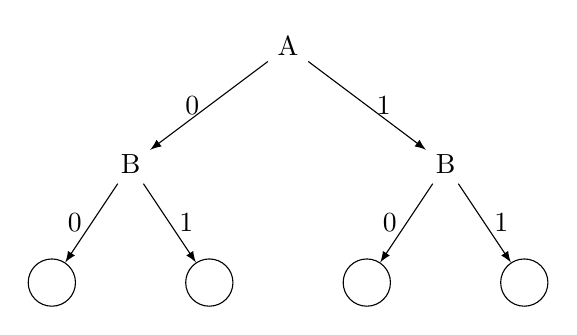
\begin{tikzpicture}[level distance=1.5cm,
%   every node/.style={circle,draw,minimum size=8mm,inner sep=0pt},
  edge from parent/.style={draw,-latex},
  level 1/.style={sibling distance=4cm},
  level 2/.style={sibling distance=2cm}
  ]
\node (A) {A}
  child {node (B1) {B}
    child {node[circle,draw,minimum size=6mm,inner sep=0pt,fill=white] {}
      edge from parent node[left] {0}
    }
    child {node[circle,draw,minimum size=6mm,inner sep=0pt,fill=white] {}
      edge from parent node[right] {1}
    }
    edge from parent node[left] {0}
  }
  child {node (B2) {B}
    child {node[circle,draw,minimum size=6mm,inner sep=0pt,fill=white] {}
      edge from parent node[left] {0}
    }
    child {node[circle,draw,minimum size=6mm,inner sep=0pt,fill=white] {}
      edge from parent node[right] {1}
    }
    edge from parent node[right] {1}
  };
\end{tikzpicture}
\end{center}
\end{example}

\begin{remark}
Notice that communication complexity presents a combinatorial setting to solve problems, which have much more mathematical tools compared to general complexity. Therefore, 
\end{remark}

\begin{lemma}
A protocol that sends $c$ bits has a protocol tree of depth $c$. This implies you can partition your matrix (whose rows are the possibilities of $x$ and columns $y$) into $2^c$ monochromatic rectangles. (Recall that a partition is a disjoint collection whose union is the whole thing.)
\end{lemma}

\begin{definition}
A \term{monochromatic rectangle} is a subset of the matrix $R \subseteq X \times Y$ such that if $(x,y), (x',y') \in R$, then $(x,y'),(x',y) \in R$. 
\end{definition}

\begin{example}
Consider the following matrix:
\begin{center}
    \begin{tabular}{c c}
        1 & 0 \\ 
        0 & 1
    \end{tabular}
\end{center}
This cannot be one monochromatic rectangle. However, 
\begin{center}
    \begin{tabular}{c c}
        1 & 1 \\ 
        1 & 1
    \end{tabular}
\end{center}
can be expressed as one monochromatic rectangle.
\end{example}

\begin{example}
Notice that the matrix for $\text{Eq}$ from Example \labelref{1.1} is just the identity matrix. By \labelref{1.4} there must be at least $n$ monochromatic rectangles, one for each $1$ on the diagonal. Therefore, no protocol exists that does better than $n$ bits communicated for $\text{Eq}$.
\end{example}

\begin{remark}
Notice that since we care about the worst case, that is all $x,y$, we care more about the number of rectangles, not the size of the rectangles; it is possible that our matrix is covered mostly by 1 rectangle, but many (hard) inputs can only be covered by very small rectangle.
\end{remark}

\subsection{Fooling Sets}

\begin{definition}
TODO; A \term{fooling set} is a subset $F \subseteq X \times Y$ such that if $(x,y), (x',y') \in F$ and $f: X \times Y \to {0,1}$ is the evaluation function, then either $f(x,y') \neq f(x,y)$ or $f(x',y) \neq f(x,y)$ such that it cannot be a single monochromatic rectangle.
\end{definition}

\subsection{Richness}

\begin{definition}
Define \term{richness} as a tuple $(u,v)$ describing the matrix of a protocol, particularly when $|X| < |Y|$ or vice versa. $u$ refers to the number of rows that have $v$ $1$s. Together with the size of $X,Y$, and the number of $1$s in the matrix, you can give an upper bound on the maximum size of a 1-monochromatic-rectangle and therefore a lower bound on the number of monochromatic rectangles (and thus communication complexity in general).
\end{definition}

\begin{example}
Consider the following matrix:
\begin{center}
    \begin{tabular}{c c c c}
        1 & 1 & 0 & 0 \\ 
        1 & 1 & 0 & 1 \\
        0 & 0 & 0 & 0 \\
        0 & 1 & 0 & 0
    \end{tabular}
\end{center}
The above has richness $(3,1), (2,2), (1,3)$. This tells us a maximum size of a 1-monochormatic rectangle (in particular, 2 by 2), which just happens to be tight here.
\end{example}

\begin{remark}
Note that rectangles and richness easily extend to relations, where there may be more than one possible input (for example, consider indexed sets $X$, $Y$ and finding $i$ where $X_i = Y_i$).
\end{remark}

\subsection{Computing Functions and Relations}

\begin{definition}
Define the \term{computational complexity} of $g: X \times Y \to \{0,1\}$ denoted $\CC(g)$ is the minimum depth of the protocol tree of $g$. Define $P(g)$ as the minimum number of leaves, equivalently, the number of monochromatic triangles of the protocol tree.
\end{definition}

\begin{lemma}
$P(g) \leq 2^{\CC(g)}$. Also, $\sqrt{\CC(g)} \leq \log_2 P(g) \leq \CC(g)$.
\end{lemma}

\begin{example}
Suppose $g : X \times Y \to \{0,1\}$ and $g$ requires $c$ bits of communication. Suppose we wish to compute $g^m$. If $g$ is a function, $\CC(g^m) = \CC(g)^m$ is an open problem. If $g$ is a relation, you cannot do this. TODO; See book why.
\end{example}

\begin{theorem}
$P(g^m) = P(g)^m$.
\end{theorem}

\begin{remark}
We can study the number of leaves but not the depth...
\end{remark}

